% Some LaTeX commands I define for my own nomenclature.
% If you have to, it's better to change nomenclature once here than in a 
% million places throughout your thesis!


%======================================================================
\chapter{Data}
%======================================================================

\section{Survey Introduction}
This research is based on an Internet-based survey of Foreign visitors and Japanese who have visited Tokyo, conducted by the Economic and Social Research Institute. A total of 1800 people were surveyed, including 300 people from each country. The detailed information is shown in \#Table 1. 

\section{Question description}
The survey was divided into 6 items, the detailed description and available answers of each question in \#Table 2. The first item, FQ1-FQ7, consists of seven demographic questions, including nationality, gender, age, travel experience, and Japanese proficiency. The second to fourth items are Q1-Q10, which includes disaster consciousness, disaster training experience, earthquake experience, earthquake knowledge, and disaster response knowledge. The fifth item is Q11-Q14, which is about respondents' response actions in four scenarios during the "Tokyo Metropolitan Earthquake." ( I'll go over scenarios in 3.3). The sixth item is Q15-Q17, which is about respondents' attitudes toward Safety Tips, including respondents' usage experiences as well as their perceptions of Safety Tips.

\section{Scenario description}
In item No.5, all respondents should answer their Information seeking and evacuation behavior in each of the following scenarios. There are two types of differences between the scenarios, resulting in four different scenarios. The first type of difference is network-related and is divided into "Telephone/internet is available" and "Telephone/internet is not available (A temporary power outage occurs)". The second type of difference is location-related, divided into "Staying in a tourist attraction" and "Moving by public transportation". Thus the 4 scenarios are shown in \#Table 3.

In order to answer response actions during the disaster, all respondents were requested to watch a simulation video of the "Tokyo Metropolitan Earthquake". The video is provided by the Cabinet Office,  and the simulation video has been translated into their native languages. The simulation video shows an earthquake of magnitude 7.3 that occurred in the southern part of Tokyo, happened on a winter evening in the year 20xx, and in order to show the damage, the landscape is represented brighter than it actually is. After watching the video, the respondents were requested to select 5 response actions with an order in each of the scenarios. Some screenshots of the simulation video are shown in Figure~\ref{fig5}.

In the pre-survey, we collected some common evacuation behaviors of foreign visitors and Japanese people. It's worth noting that selections 1-7 are only available in scenarios 1 and 3 because they require a phone/internet connection. \#Table 4 contains a list of all selections as well as a detailed description of each one.

\begin{figure*}[h]
  \begin{subfigure}{0.32\textwidth}
    \centering
    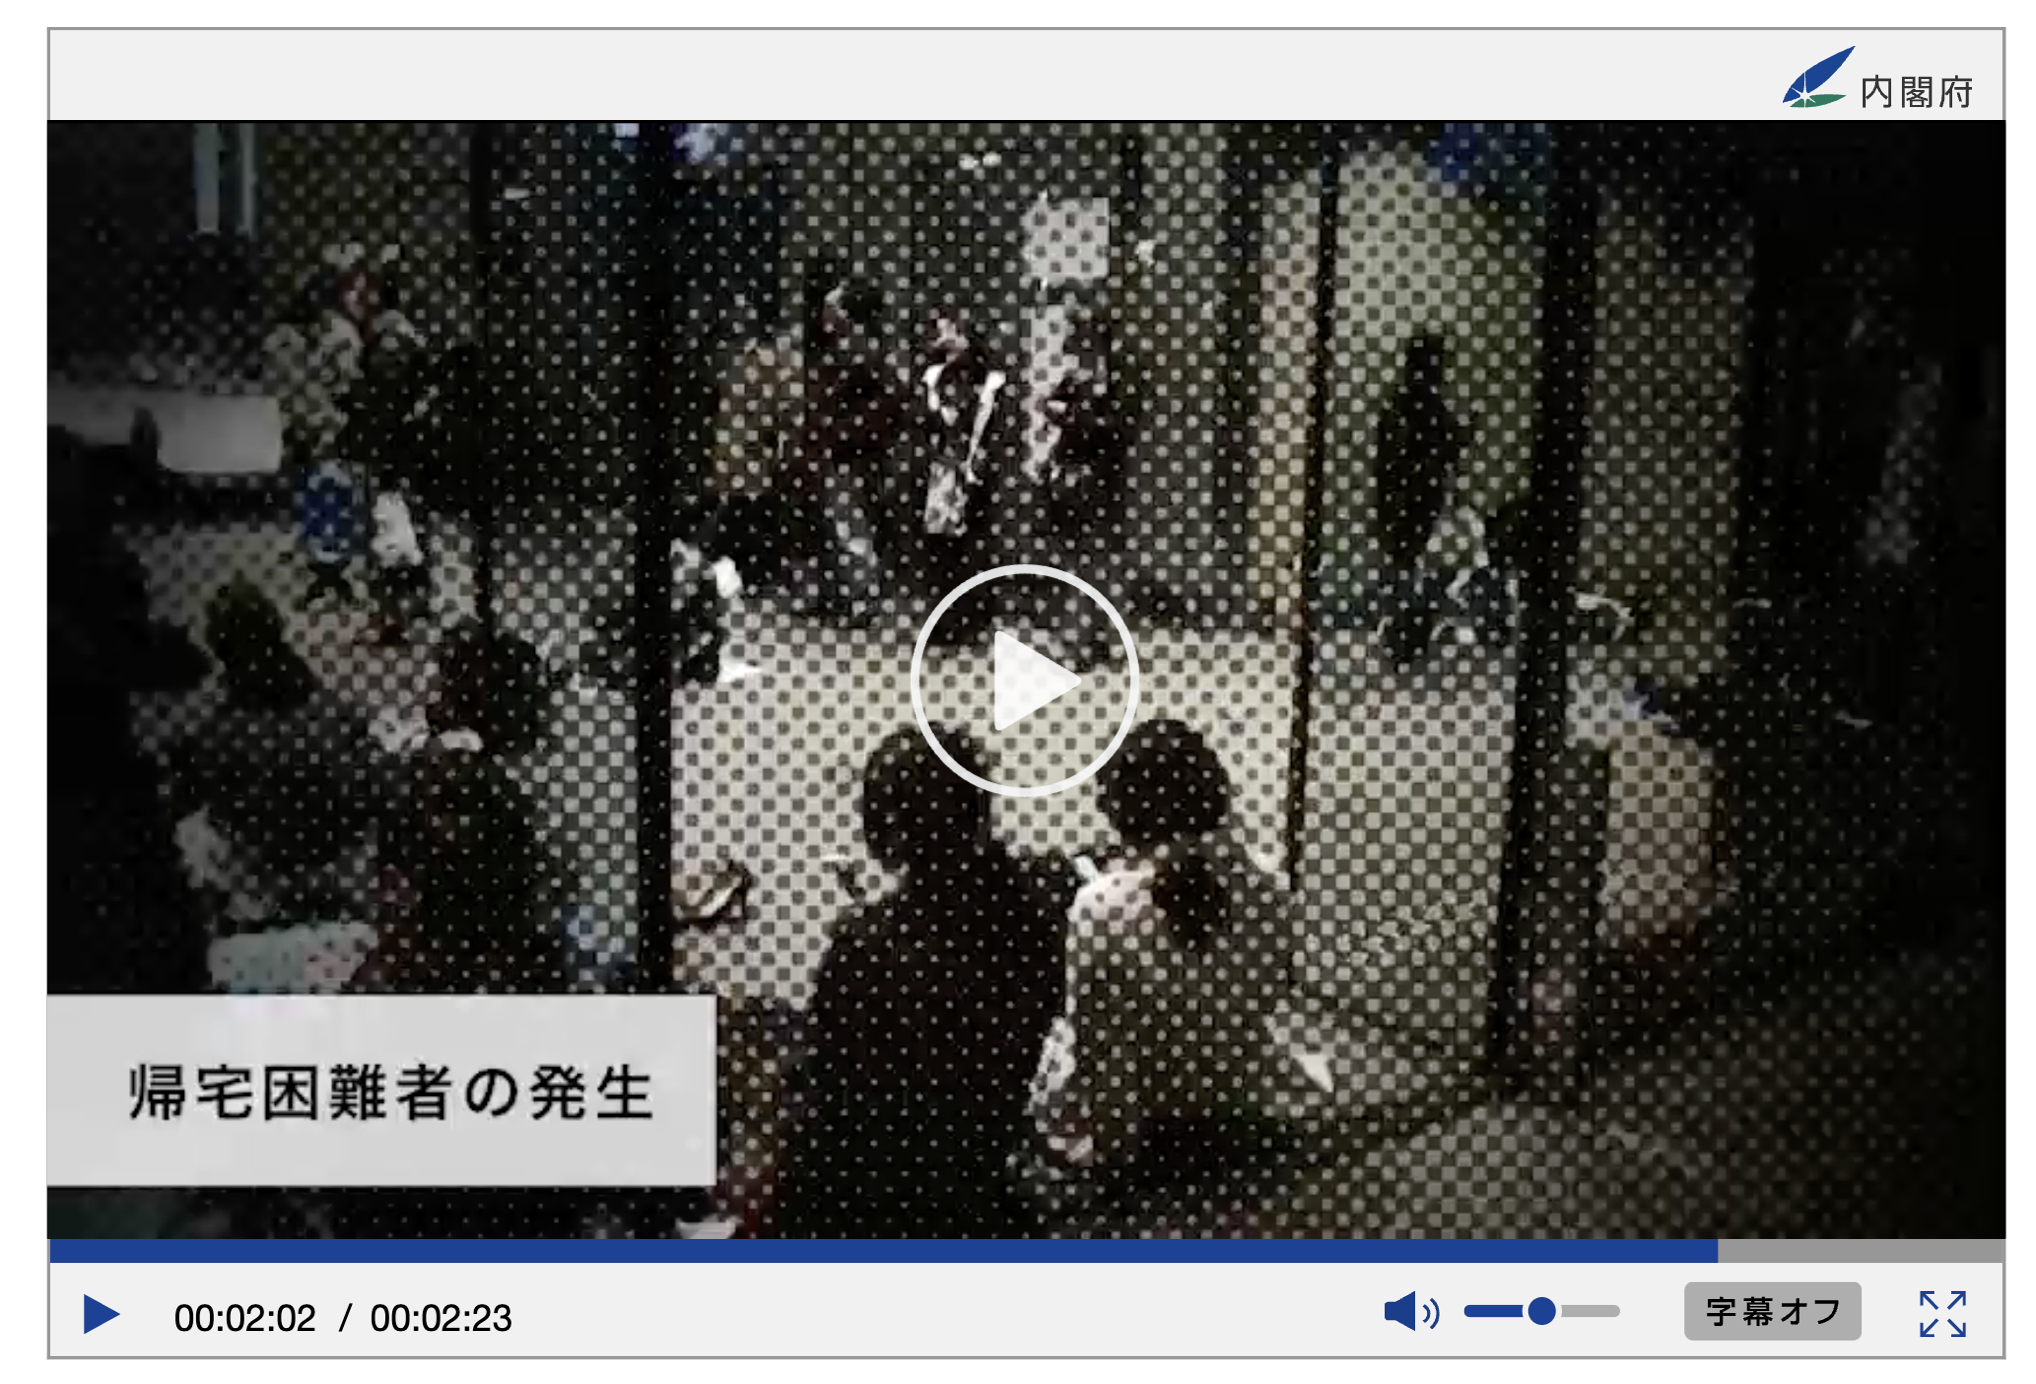
\includegraphics[width=\textwidth]{Figure/Figure5a.jpg}
    \caption{Difficulty in returning home}
    \label{fig5a}
  \end{subfigure}\hfill
  \begin{subfigure}{0.32\textwidth}
    \centering
    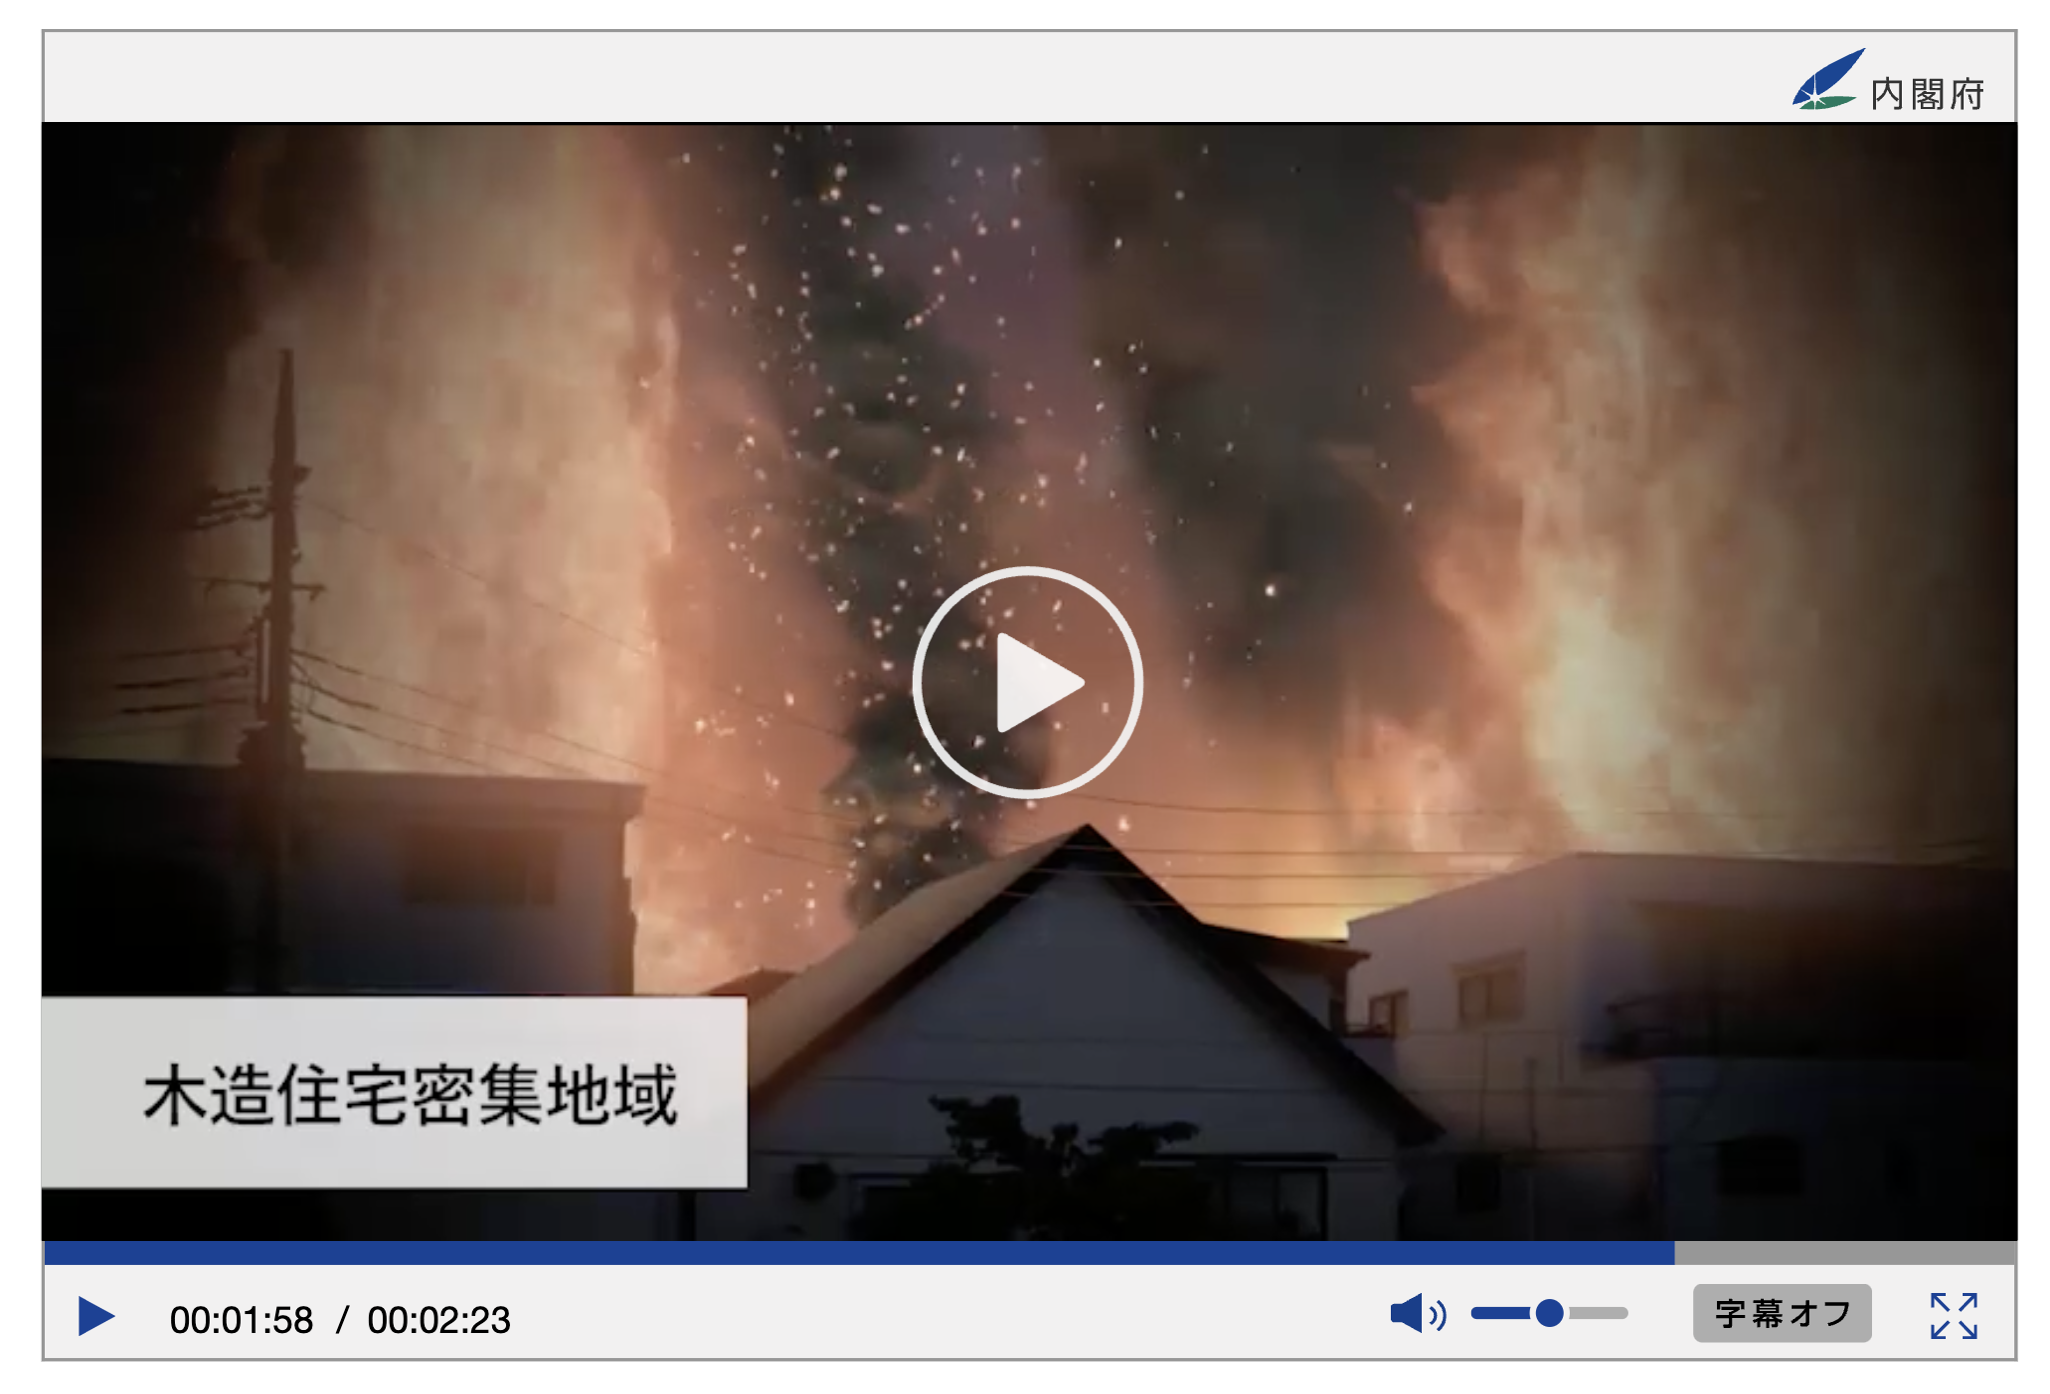
\includegraphics[width=\linewidth]{Figure/Figure5b.jpg}
    \caption{Dense area of wooden houses; Fire occurred easily}
    \label{fig5b}
  \end{subfigure}\hfill
  \begin{subfigure}{0.32\textwidth}
    \centering
    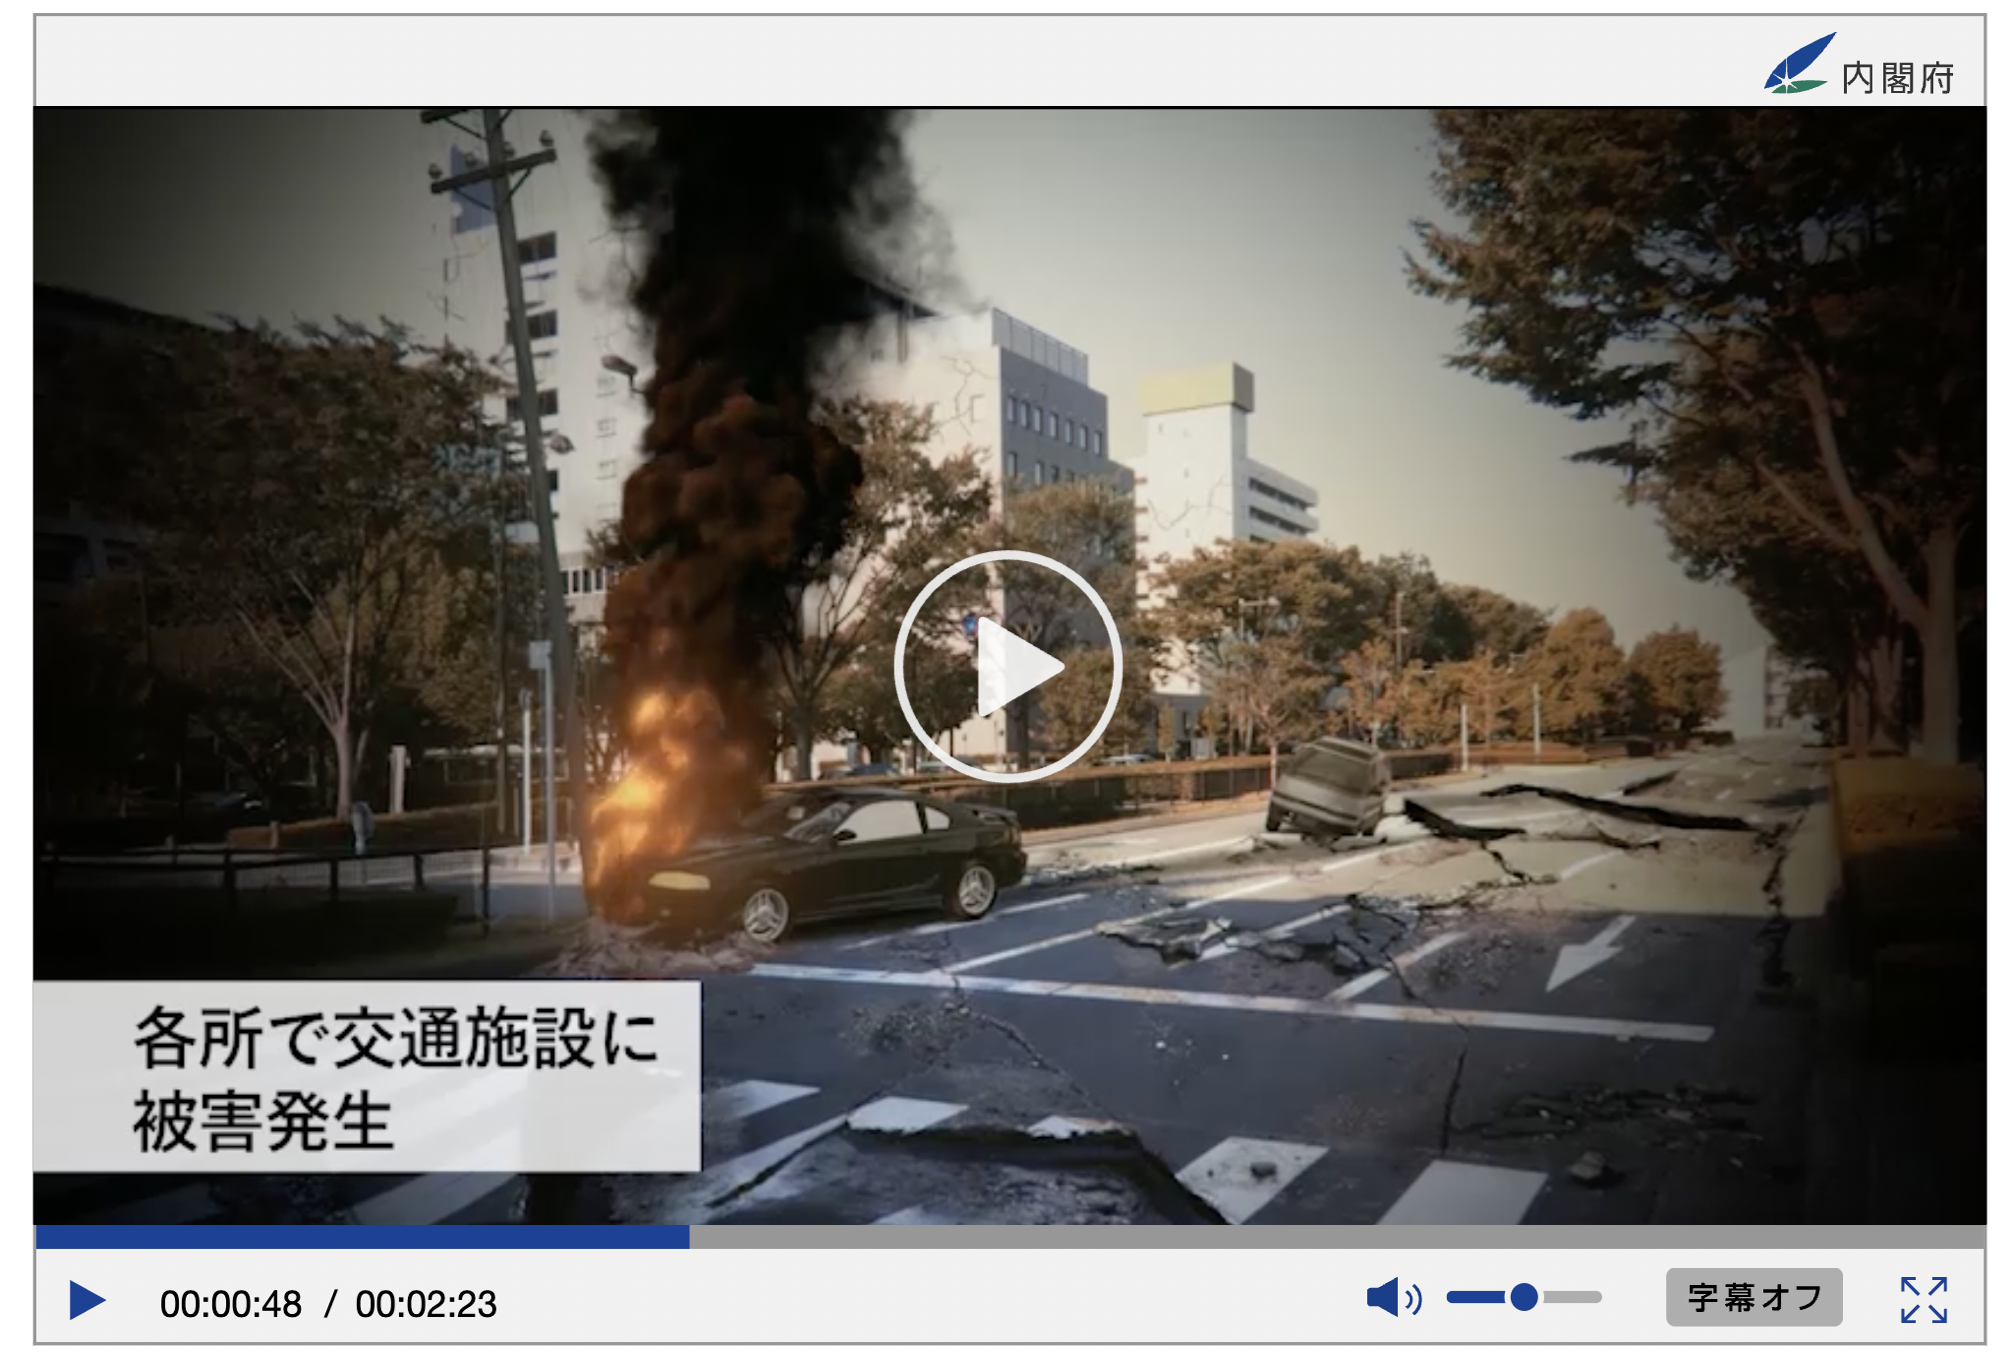
\includegraphics[width=\linewidth]{Figure/Figure5c.jpg}
    \caption{Damage to transportation facilities in many places}
    \label{fig5c}
  \end{subfigure}\hfill
  \begin{subfigure}{0.32\textwidth}
    \centering
    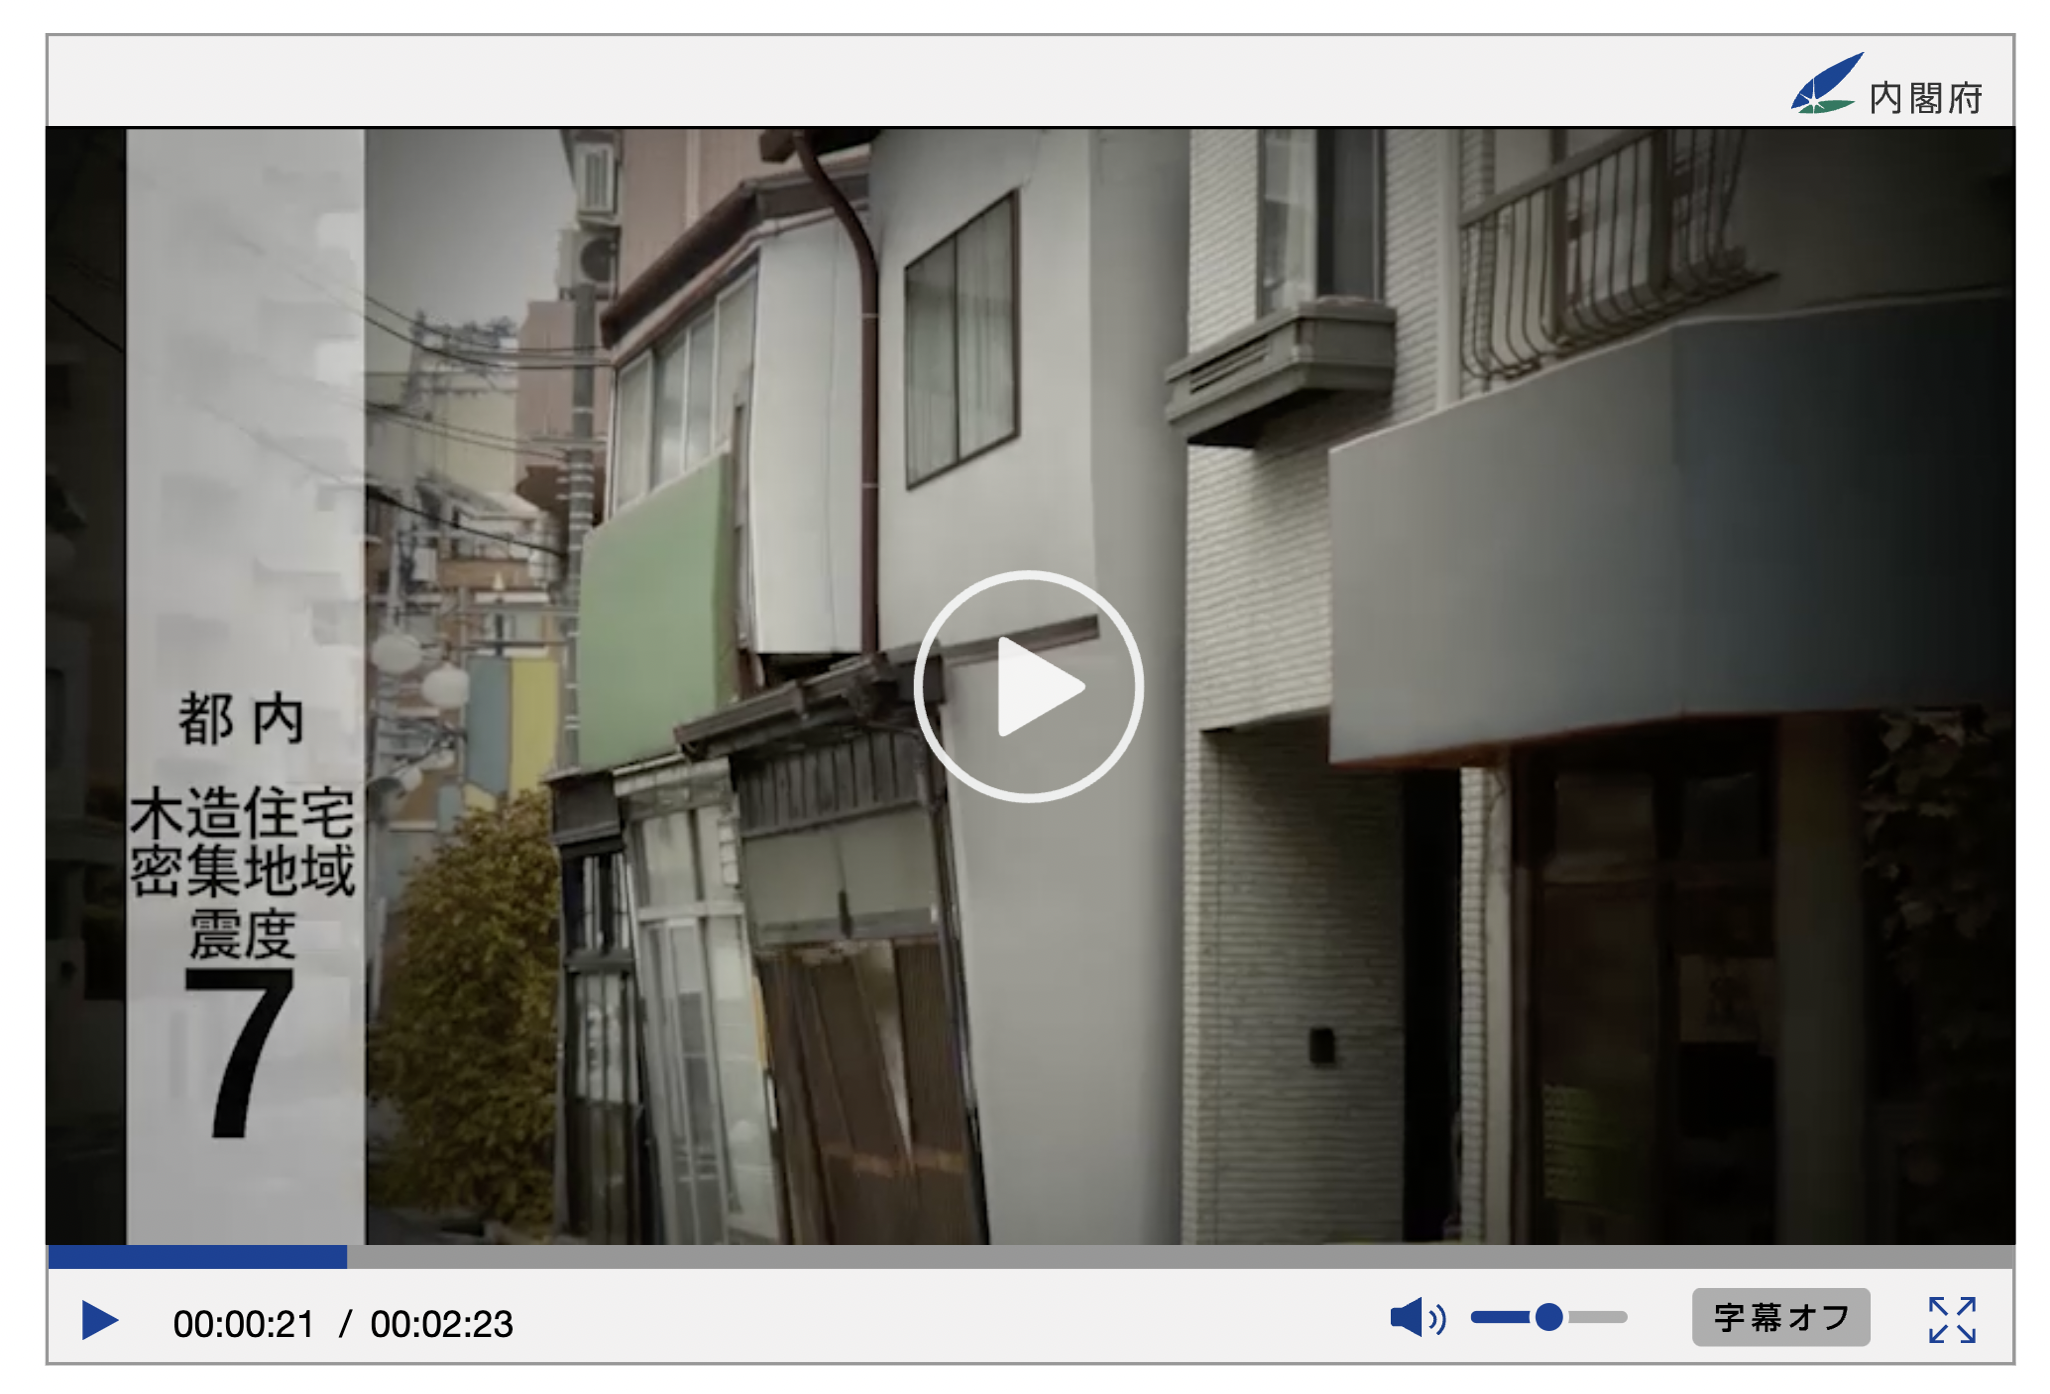
\includegraphics[width=\linewidth]{Figure/Figure5d.jpg}
    \caption{Tokyo-Wooden houses(Dense area); Seismic intensity 7}
    \label{fig5d}
  \end{subfigure}\hfill
  \begin{subfigure}{0.32\textwidth}
    \centering
    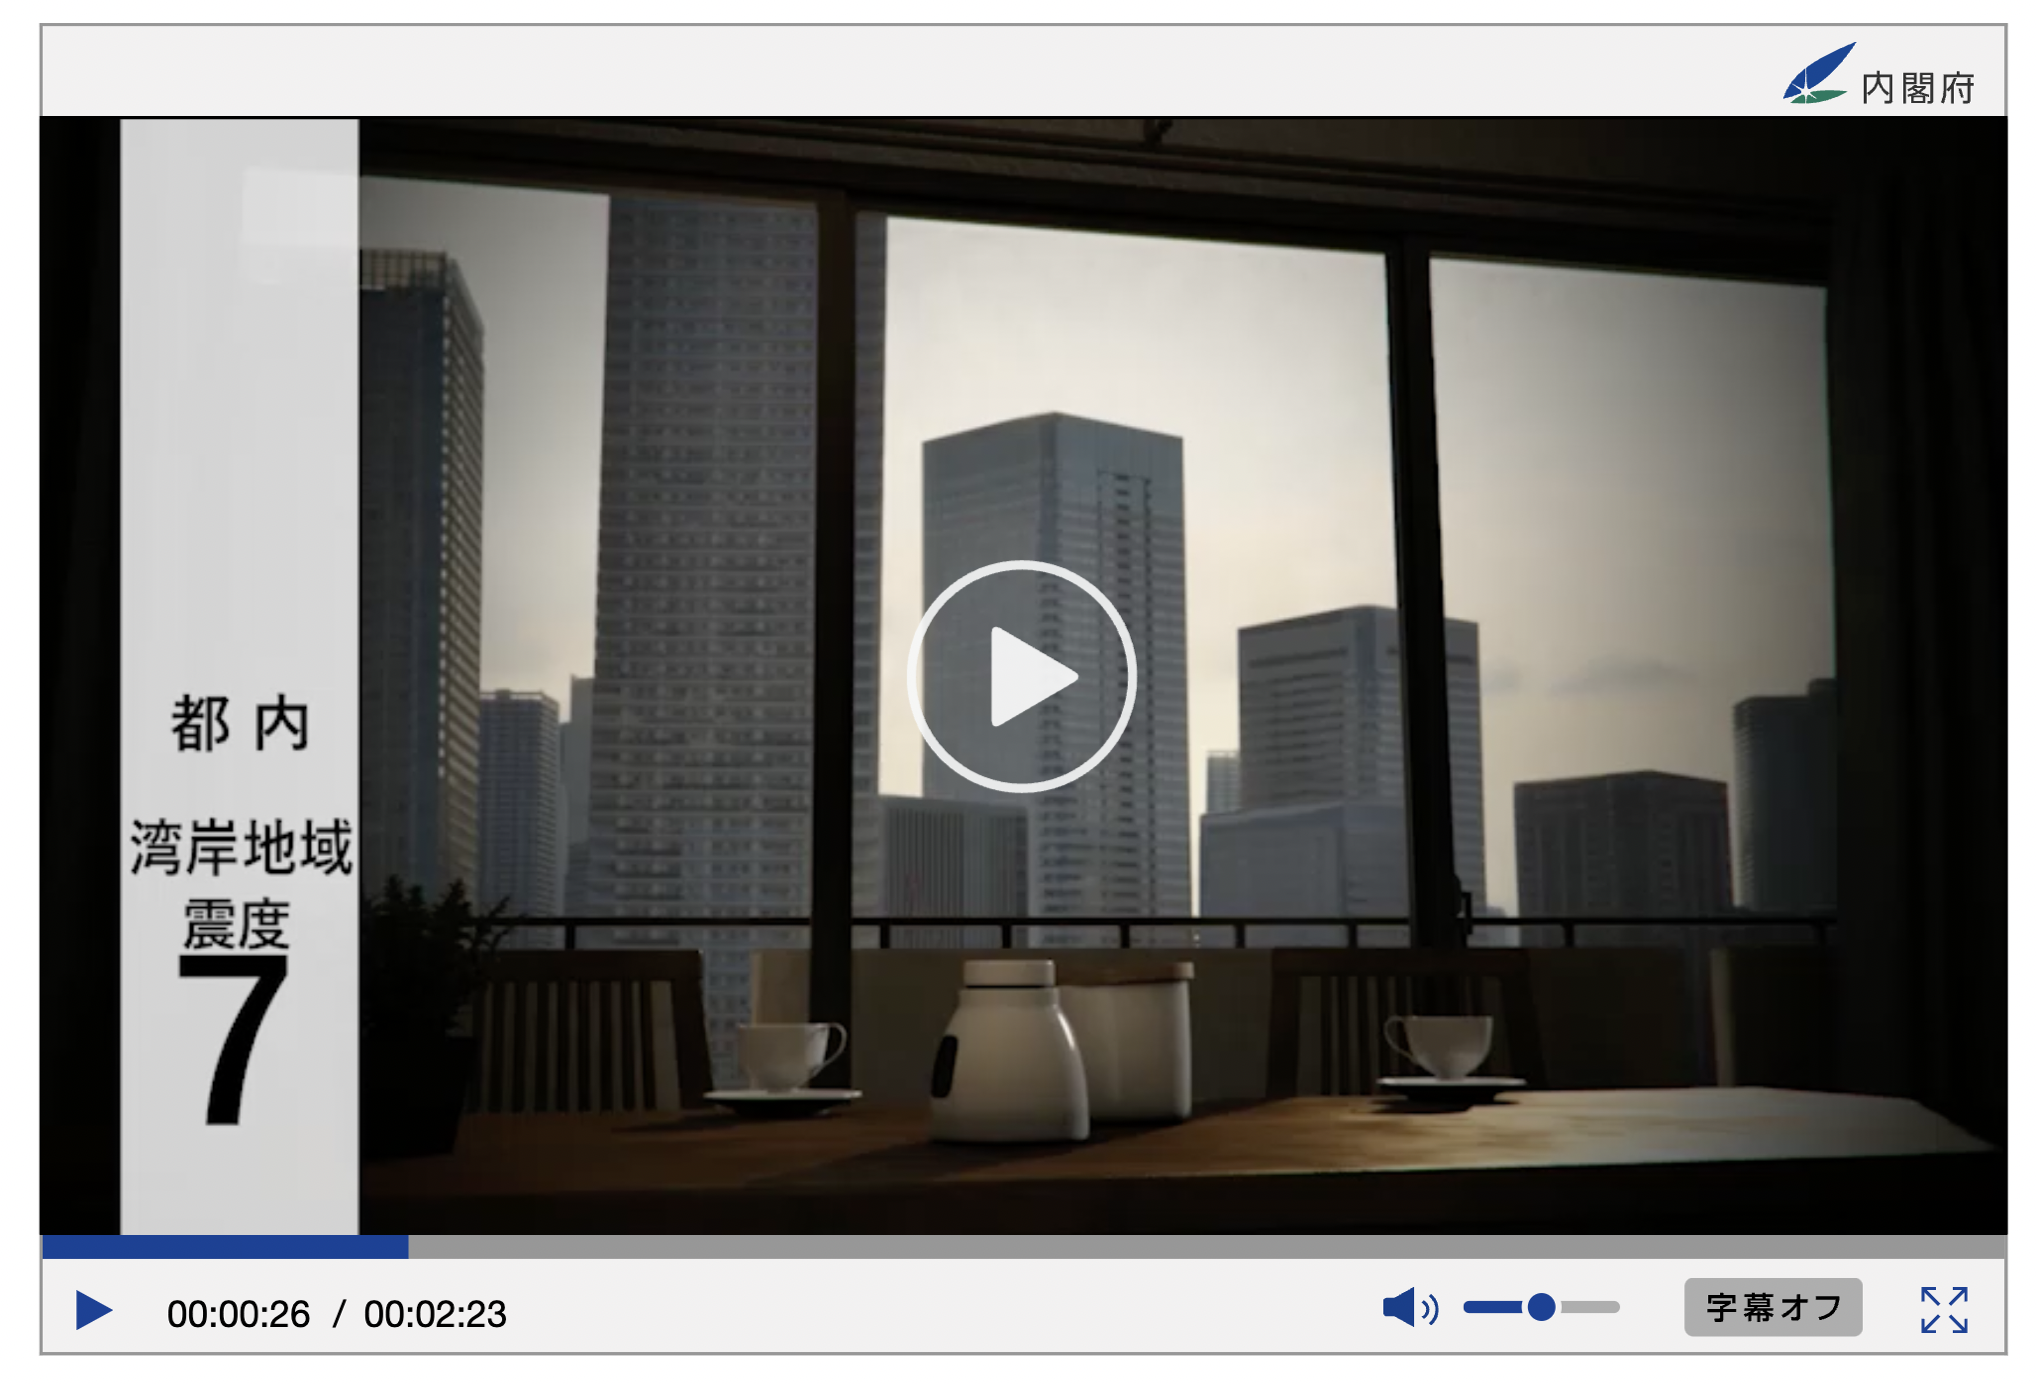
\includegraphics[width=\linewidth]{Figure/Figure5e.jpg}
    \caption{Tokyo-Bay Area; Seismic intensity 7}
    \label{fig5e}
  \end{subfigure}\hfill
  \begin{subfigure}{0.32\textwidth}
    \centering
    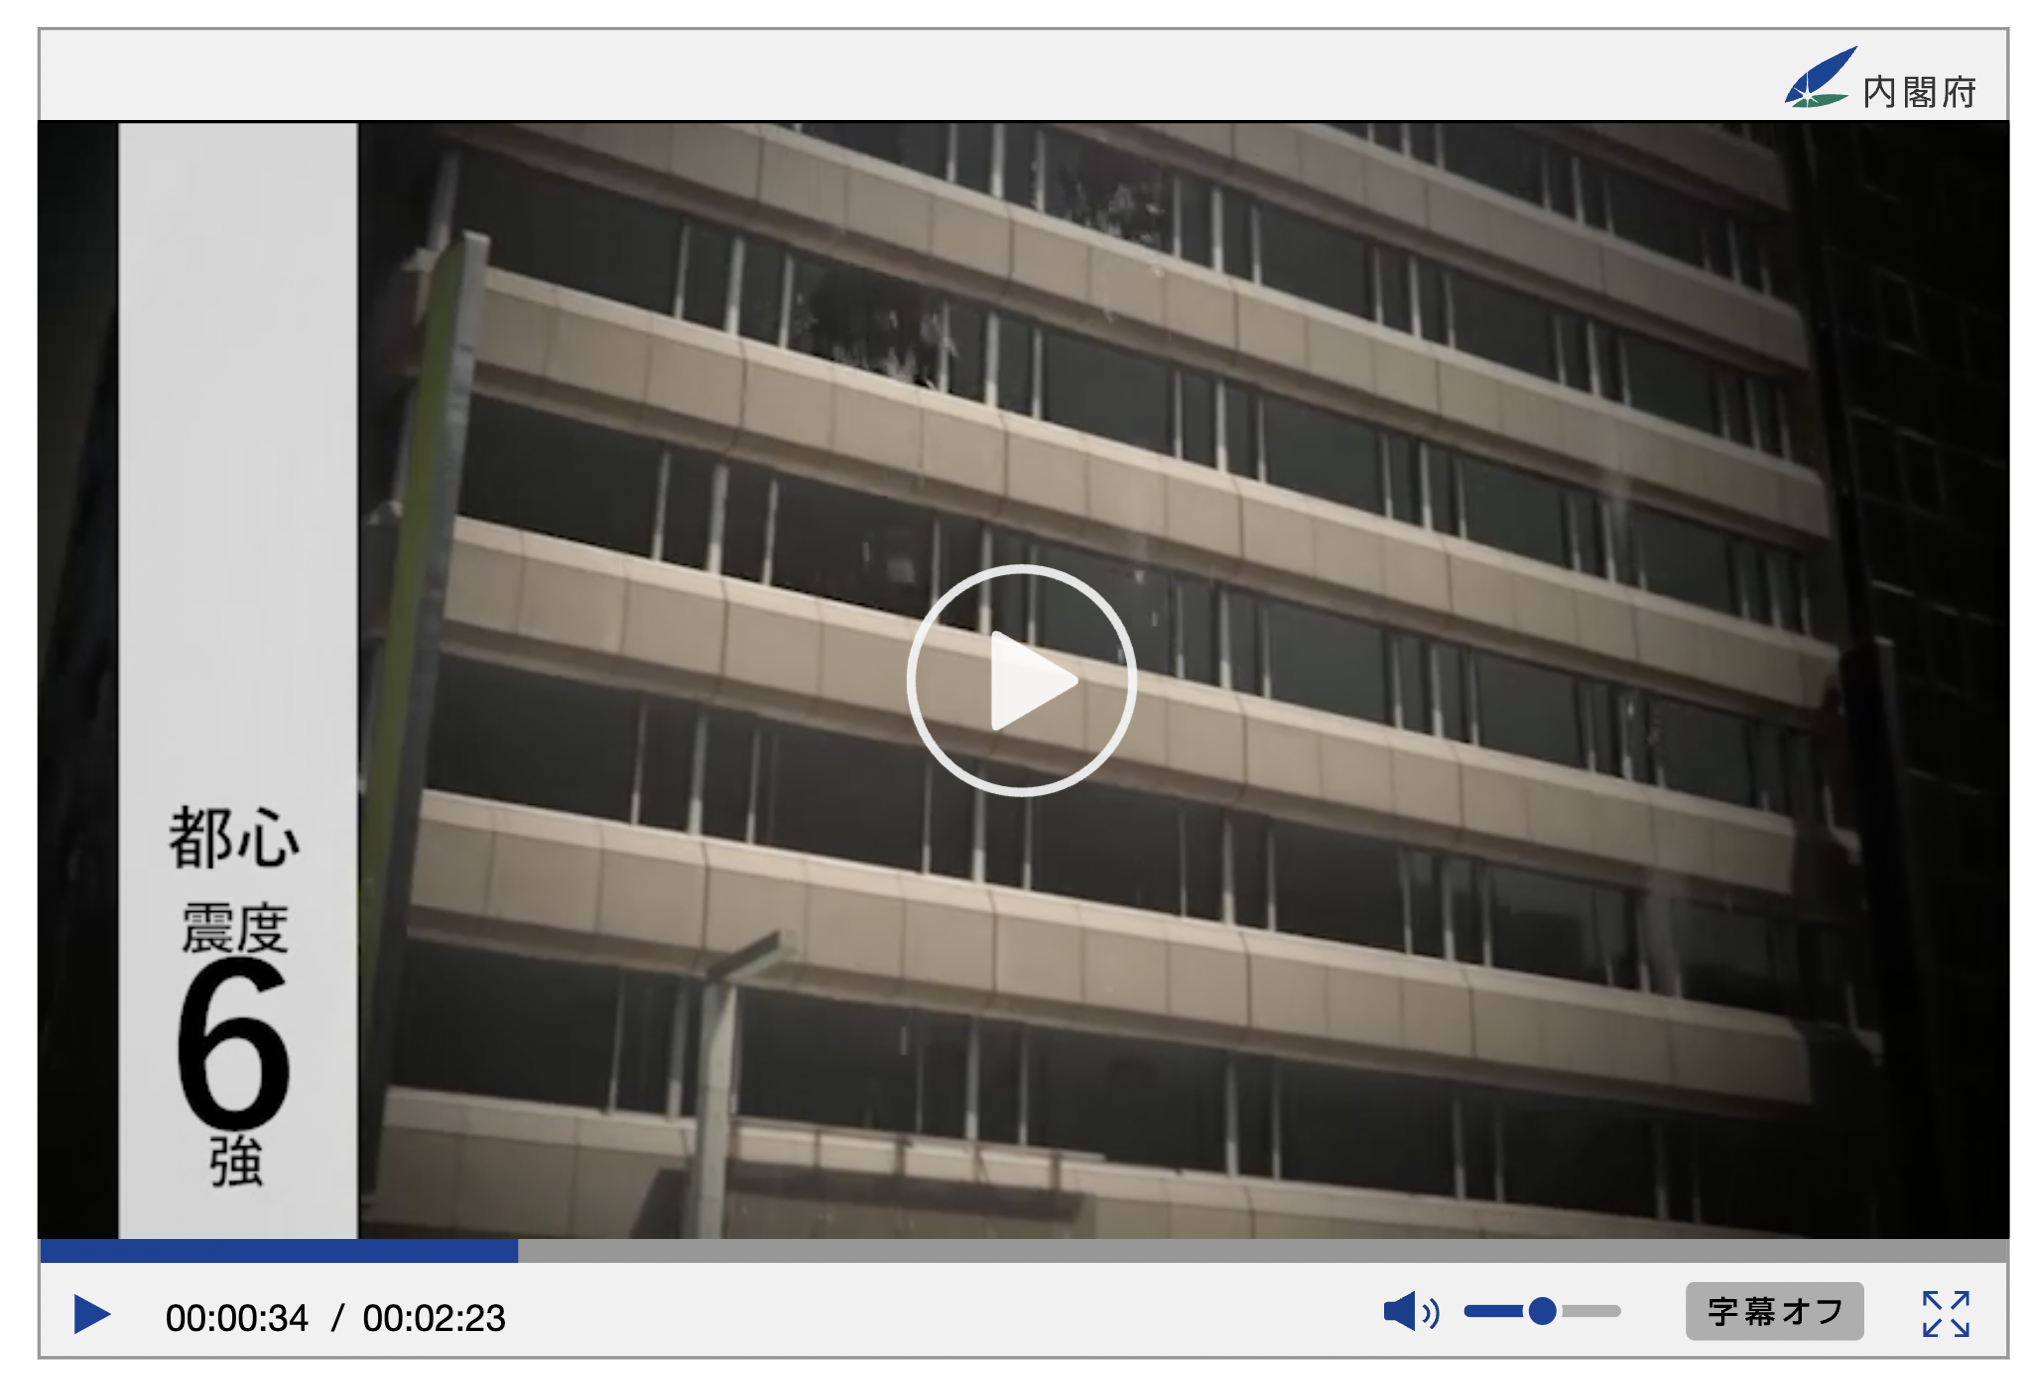
\includegraphics[width=\linewidth]{Figure/Figure5f.jpg}
    \caption{Tokyo; Seismic intensity 6-}
    \label{fig5f}
  \end{subfigure}
  \begin{subfigure}{0.32\textwidth}
    \centering
    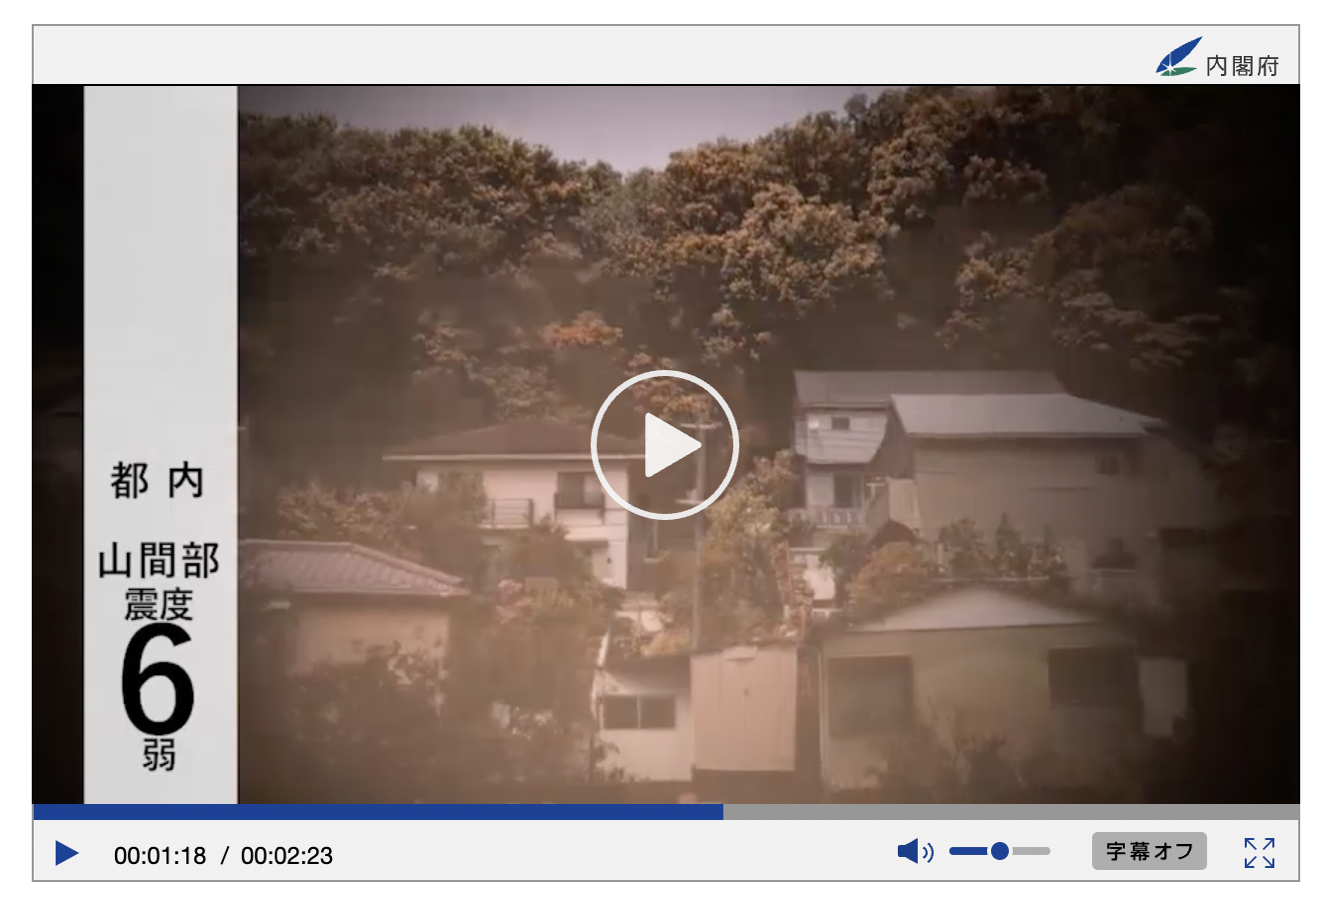
\includegraphics[width=\linewidth]{Figure/Figure5g.jpg}
    \caption{Tokyo-Mountainous region; Seismic intensity 6+}
    \label{fig5g}
  \end{subfigure}
  \centering
  \caption[Simulation video of “Tokyo Metropolitan Earthquake”.]{Simulation video of “Tokyo Metropolitan Earthquake”.\protect\footnotemark }
  \label{fig5}
\end{figure*}
 \footnotetext{http://wwwc.cao.go.jp/lib\_012/syuto\_02.html}